\documentclass[12pt]{article}

\usepackage[utf8]{inputenc}
\usepackage[margin=1in]{geometry}
\renewcommand{\baselinestretch}{1}
\usepackage{indentfirst}

\usepackage{amsmath, amssymb}

\usepackage{graphicx}
\usepackage{float}
\graphicspath{{./figs/}}

\begin{document}

\begin{center}\begin{LARGE}
\textbf{Assignment 2: Results/Description}
\end{LARGE}\end{center}

\section*{Problem 1}

Let $\{f_i(\boldsymbol{x})\}$ be the system of nonlinear equations for which
we wish to find a root. Then we may introduce $\boldsymbol{f}(\boldsymbol{x})$
comprised of components $f_i$ that satisfies
$$
\begin{aligned}
\boldsymbol{f}(\boldsymbol{x})
= \boldsymbol{0}.
\end{aligned}
$$
Let $\boldsymbol{\xi}$ be the root of $\boldsymbol{f}(\boldsymbol{x})$. Then
one may Taylor expand around $\boldsymbol{\xi}$ so that
$$
\begin{aligned}
0
&= f_i(\boldsymbol{\xi}) \\
&= f_i(\boldsymbol{x}) + \sum_j (\xi_j - x_j) \partial_j f_i(\boldsymbol{x})
  + \mathcal{O}(|\boldsymbol{\xi} - \boldsymbol{x}|^2) \\
\Rightarrow
\boldsymbol{0}
&\approx \boldsymbol{f}(\boldsymbol{x})
  + \boldsymbol{J}(\boldsymbol{x}) (\boldsymbol{\xi} - \boldsymbol{x})
\end{aligned}
$$
for $J_{ij} = \partial_j f_i(\boldsymbol{x})$. Here we assume we may neglect
the quadratic and higher order terms, assuming
$|\boldsymbol{\xi} - \boldsymbol{x}|$ is small. Therefore, rearranging this
gives
$$
\begin{aligned}
\boldsymbol{\xi}
&\approx \boldsymbol{x} - \boldsymbol{J}^{-1}(\boldsymbol{x})
    \boldsymbol{f}(\boldsymbol{x}),
\end{aligned}
$$
assuming $\boldsymbol{J}$ is invertible. Using iteration to make this
approximation converge to the true value of $\boldsymbol{\xi}$, this means
$$
\begin{aligned}
\boldsymbol{x}_{k+1}
&= \boldsymbol{x}_k - \boldsymbol{J}^{-1}(\boldsymbol{x}_k)
    \boldsymbol{f}(\boldsymbol{x}_k).
\end{aligned}
$$
for iteration index $k$.

\section*{Problem 2}

\subsection*{(a)}

I've written this program to solve the system of equations, which is the
attached ``./bin/myroot". This should compile with \texttt{make} as shown
below.

\begin{figure}[H]
    \centering
    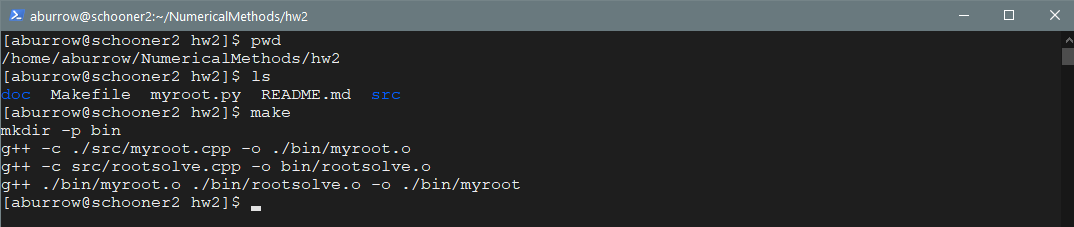
\includegraphics[width=1.0\textwidth]{compile}
    \label{fig:compile}
\end{figure}

This program makes use of the Newton-Raphson method derived in Problem 1. Here
I have analytically found $\boldsymbol{J}(\boldsymbol{x})$ with
$\boldsymbol{x} = (x, y)^\mathsf{T}$ to be
$$
\begin{aligned}
\boldsymbol{J}(\boldsymbol{x})
&=
\begin{pmatrix}
\cos(x + y) & \cos(x + y) \\
-\sin(x - y) & \sin(x - y) \\
\end{pmatrix}
\end{aligned}
$$
and for the sake of computation speed in the program I analytically solve for
$\boldsymbol{J}^{-1}(\boldsymbol{x}) \boldsymbol{f}(\boldsymbol{x})$,
$$
\begin{aligned}
\boldsymbol{J}^{-1}(\boldsymbol{x}) \boldsymbol{f}(\boldsymbol{x})
&= \frac{1}{2 \cos(x + y) \sin(x - y)}
\begin{pmatrix}
\sin(x - y) & -\cos(x + y) \\
\sin(x - y) & \cos(x + y) \\
\end{pmatrix}
\begin{pmatrix}
\sin(x + y) \\
\cos(x - y) \\
\end{pmatrix} \\
&= \frac{1}{2}
\begin{pmatrix}
\tan(x + y) - \cot(x - y) \\
\tan(x + y) + \cot(x - y) \\
\end{pmatrix}.
\end{aligned}
$$

The main problem here is determining the initial approximation
$\boldsymbol{x}_0$. Because we have periodic functions, we know analytically
that there will be an infinite number of roots that are separated by integer
multiples of $\pi$. Therefore, we may want to limit the roots to some region in
$\boldsymbol{x}$ space. This is easiest done using the starting point of this
Newton-Raphson method. Because the Jacobian is found analytically, the root
found will effectively be that closest in $\boldsymbol{x}$ space to the
starting guess. In general, one must be careful of their choice of
$\boldsymbol{x}_0$, as the root found is highly dependent on it when there are
multiple roots of the function. If we want to find more roots with this method,
more starting points must be sampled to find all the local minima. It is also
easier to find what the relevant starting points are if you can plot the
function and look into the region you want.

For the function in this problem, we know there are 2 unique roots within the
unit circle $|x|, |y| < \pi$ (due to $x$-$y$ symmetry). They are also
spaced out by $\pi$, however in order for $\boldsymbol{J}$ to be invertible,
$x$ and $y$ must not differ by $n\pi$ for some $n \in \mathbb{Z}$. Therefore,
we find the roots by checking two different starting points between $|x|, |y| <
\pi / 2$ and $\pi / 2 < |x|, |y| < \pi$.

For example, with $\boldsymbol{x}_0 = (-1, 1)^\mathsf{T}$, where $|x|, |y| <
\pi / 2$, the program yields a root which is effectively $x=\pi/4$ and
$y=-\pi/4$:
\begin{figure}[H]
    \centering
    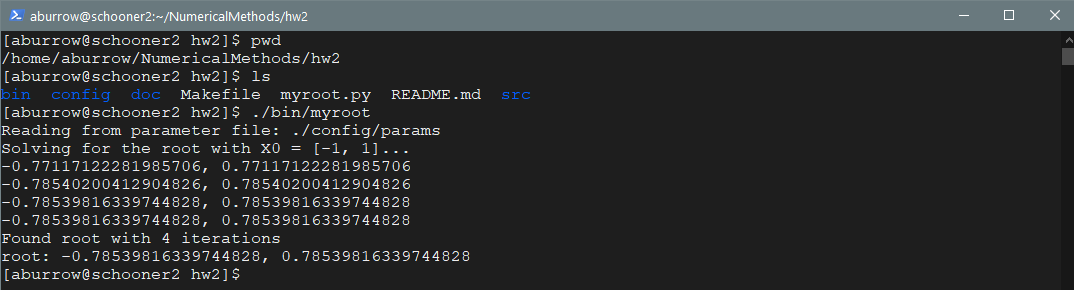
\includegraphics[width=1.0\textwidth]{root1}
    \label{fig:root1}
\end{figure}
When $\pi / 2 < |x|, |y| < \pi$, where as an example $\boldsymbol{x}_0 =
(-2, 2)^\mathsf{T}$, the other root ($x=3\pi/4$ and $y=-3\pi/4$) is
found:
\begin{figure}[H]
    \centering
    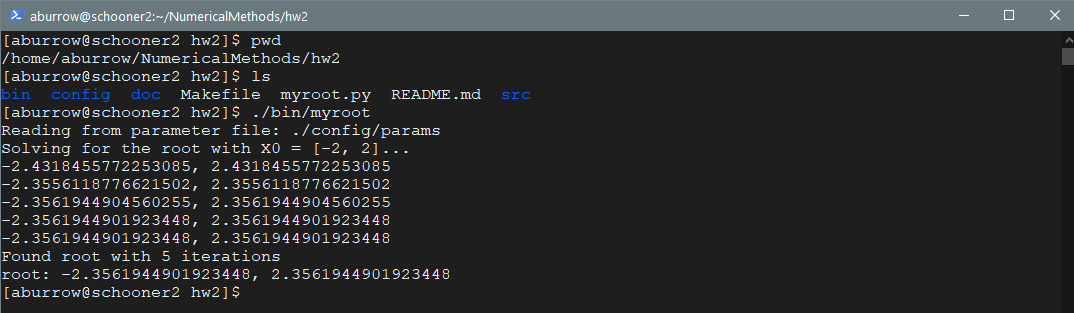
\includegraphics[width=1.0\textwidth]{root2}
    \label{fig:root2}
\end{figure}

Numerically, we find these roots to be
$$
\begin{aligned}
\begin{pmatrix}
-0.78539816339744828 \\ 0.78539816339744828
\end{pmatrix}
\end{aligned}
$$
and
$$
\begin{aligned}
\begin{pmatrix}
-2.3561944901923448 \\ 2.3561944901923448
\end{pmatrix}.
\end{aligned}
$$
Each estimate of the root is shown, and a final value is reached when the
difference between the new and old estimates are machine zero.

\subsection*{(b)}

I solved this problem in Python as well (``./myroot.py''), using SciPy's
\texttt{scipy.optimize.fsolve} function. Using the same two sets of initial
conditions, it was able to solve the same roots to the same (double) precision:
\begin{figure}[H]
    \centering
    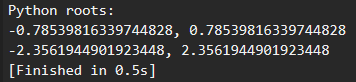
\includegraphics[width=1.0\textwidth]{python}
    \label{fig:python}
\end{figure}

Typically Python can be used to perform the same calculations for these simple
problems (as we saw, it only takes ~5 iterations to find a decent result). This
is true especially when you are able to vectorize the problem so that one may
take advantage of Numpy's C-optimized functionality. However its flexibility
makes it quite burdensome to perform heavy calculations with more complicated
problems.

\end{document}
